\chapter{Object Reconstruction}
\label{chap:objects}

In this chapter the physics objects necessary to be able to perform searches with \Pgt leptons
in the final state, and how they are reconstructed in \ac{CMS}, will be discussed. The 
descriptions correspond to the algorithms as used during Run 2. Where there are differences
between the algorithms used in Run 1 and Run 2 this will be discussed at the end
of the relevant section.

\section{\acl{PF}}
\label{sec:objects_pf}
All stable particles are reconstructed and identified using the \ac{PF} algorithm \cite{cms-pf-2009,cms-pf-2010-1,cms-pf-2010-2}, which
combines the information from all of the different subdetectors of \ac{CMS}. This makes
the identification of particles, and determination of position and momentum, as precise
as possible. All of these particles are then used to build for example jets, \MET and hadronically
decaying taus.

The \ac{PF} algorithm starts from charged particle tracks measured
by the inner tracker, muon tracks measured in the muon system, and 
energy deposits in the calorimeters. These energy deposits are combined
using a clustering algorithm, so that stable neutral particles can be identified,
separated from charged hadrons, and electrons and all Bremsstrahlung photons
can be reconstructed. Clustering is performed separately in the \ac{ECAL} barrel,
\ac{ECAL} endcaps, first and second \ac{PS} layers, \ac{HCAL} barrel and \ac{HCAL} endcaps, with no 
clustering employed in the \ac{HF}.
%And to aid energy measurement of charged hadrons for which
%tracks were low quality, or high pT
The clustering algorithm used for \ac{PF} starts from \textit{cluster seeds},
calorimeter cells with local energy maxima. Topological clusters are built by 
merging neighbouring cells into the cluster, provided that the cells
being merged in contain a certain minimum energy.
The threshold is 800 MeV in the \ac{HCAL} and two standard deviations above the
expected noise level in the \ac{ECAL}, meaning 80 MeV in the barrel and up 
to 300 MeV in the endcaps. Cell energies can be shared between multiple
\ac{PF} clusters, depending on the distance between a cell and the centre of the cluster.

Any given particle will usually give rise to multiple \ac{PF}
elements in the different subdetectors. To provide full reconstruction
of each particle, and avoid double counting,  the next step in the
\ac{PF} algorithm is to link the different elements. This is
achieved by defining a distance parameter between any two \ac{PF} elements
in the event, which quantifies the link quality. Directly and indirectly
linked elements are considered as input blocks to the reconstruction and
identification algorithm. Links between charged tracks and calorimeter
clusters are established by extrapolating the track from its last measured
tracker hit to the \ac{PS} layers, the \ac{ECAL} and the \ac{HCAL}. %in ECAL to expected maximum of a 
%typical longitudinal electron shower profile and in the HCAL at a depth correspnding to one interaction
%length.
If the extrapolated track position is within the boundaries of the cluster, plus the size
of one cell in each direction to account for gaps between cells and multiple scattering, the
track is said to be linked to the calorimeter cluster. The distance is taken as the distance $\Delta R$ 
between the position of the cluster and the position of the track. Tangents to tracks are also extrapolated
to the ECAL from the track--tracker layer interaction points, and clusters can be 
linked to the track as a possible Bremsstrahlung photon if the extrapolated tangent
position is within the boundaries of the cluster.
Links between calorimeter clusters are made when the cluster position in the
more granular calorimeter is within the cluster of the less granular calorimeter,
with the link distance again defined as the $\Delta R$ between two cluster positions.
To determine links between charged tracks in the inner tracker and a muon track
in the muon system, a global fit between the two tracks is performed, where the link
is accepted if requirements on the maximum $\chi^2$ of this fit are met. This
$\chi^2$ also determines the distance parameter.

For each block, particles are identified following a sequence
of tests. First, if there is a link between a tracker track and a muon system track,
a particle flow muon is identified if the combined tracker and muon system
momentum is compatible with the tracker-only momentum. %within three standard deviations
The muon track is removed from the block before the next step of the algorithm.

Secondly, tracks are refitted with the \ac{GSF}, the compatibility
of the track with the already linked \ac{ECAL} clusters is assessed using
\ac{BDTs} which take several variables into account. If the candidate
passes, it is identified as a particle flow electron and the track and
\ac{ECAL} clusters are removed from the block.

Following this, remaining tracks lead to charged hadrons. The track is
given the momentum from the track fit, assuming the mass of a charged pion. If
the energy measured in the calorimeters is compatible with the momentum assigned
to the track, within uncertainties, as charged hadron is identified and the
momentum redefined by fitting the tracker and calorimeter measurements. If
the energy of the calorimeter clusters linked to the track is significantly larger than the
charged particle momentum from the track fit, additional overlapping neutral particles
are identified. If the difference between tracker momentum and calorimeter
energies is larger than the total energy registered in associated \ac{ECAL} clusters,
a particle flow photon with energy equal to the total \ac{ECAL} energy is created.
Any remaining momentum difference is assigned to a particle flow neutral hadron. If the momentum
difference is smaller than the energy registered in associated \ac{ECAL} clusters 
only a particle flow photon is created. %Justified by fact that
%in jets 25% of the energy is carried by photons while neutral hadrons
%leave only 3% of the jet energy in the ECAL. This fraction is reduced by one order of magnitued
%for taus for which decays to final states with neutral hadrons are Cabbibo suppressed to a branching ratio of 
%about a percent.

Finally, any remaining \ac{ECAL} clusters not linked to a track give
rise to particle flow photons, with any \ac{HCAL} clusters
not linked to tracks giving rise to particle flow neutral hadrons.

\section{Tracks and vertices}
\label{sec:objects_pv}

\section{Electrons}
\label{sec:objects_ele}

\section{Muons}
\label{sec:objects_muo}

\section{Jets and b-tagging}
\label{sec:objects_jets}

\subsection{Jet energy corrections}
\label{sec:objects_jets_jec}

\section{Missing energy}
\label{sec:objects_met}

\subsection{Recoil corrections}
\label{sec:objects_met_recoilcorr}

\section{Hadronic taus}
\label{sec:objects_tau}
Taus are unstable particles and they decay before reaching the detector. In 17.4 \% of 
cases they decay to muons and neutrinos, with an additional 17.8 \% decaying to electrons
plus neutrinos. The remaining 64.8 \% decay hadronically. Hadronically decaying
taus are characterised by narrow jets containing either one or three charged
particles ($\pi^{\pm}, K^{\pm}$) and 0,1, or two neutral pions. An overview
of the most common possible decay modes is given in table \ref{tab:hadronic_tau_decays}

\begin{table}[htp]
\begin{center}
\caption{Summary of hadronic tau decay modes, indicating the branching fraction, and intermediate resonances where relevant \cite{pdg-2014}.}
\begin{tabular}{@{}lll@{}}
%\toprule
\textbf{Decay mode} & \textbf{Resonance} &\textbf{Branching fraction [\%]}\\
\midrule
\Ptaupm $\rightarrow$ h$^{\pm}$\Pnut & & 11.5\%\\
\Ptaupm $\rightarrow$ h$^{\pm}$\Ppizero\Pnut& $\rho$(770) & 26.0\% \\
\Ptaupm $\rightarrow$ h$^{\pm}$\Ppizero\Ppizero\Pnut & a$_{1}$(1260) & 9.5\% \\
\Ptaupm $\rightarrow$ h$^{\pm}$h$^{\mp}$h$^{\pm}$\Pnut & a$_{1}$(1260) & 9.8\% \\
\Ptaupm $\rightarrow$ h$^{\pm}$h$^{\mp}$h$^{\pm}$\Ppizero\Pnut & & 4.8\%\\
Other modes with hadrons & & 3.2\% \\
\midrule
Total & & 64.8\% \\
%\bottomrule
\end{tabular}
\label{tab:hadronic_tau_decays}
\end{center}
\end{table}

\subsection{Identification}
\label{sec:objects_tau_id}
Hadronic tau decays are reconstructed using the \texttt{hadrons plus strips} (HPS) algorithm~\cite{cms-tau-run1,cms-tau-2015}, 
which is seeded by jets clustered from \ac{PF} candidates, using the anti-\kT algorithm with a distance parameter $\Delta R = 0.4$. 
As table \ref{tab:hadronic_tau_decays}
shows, 60\% of hadronic tau decays contain at least one \Ppizero in the final state. There is a high
probability that photons from $\Ppizero \rightarrow \Pphoton \Pphoton$ decays convert to
\APelectron \Pelectron pairs in the tracker volume, which are bent in the magnetic field and 
therefore cause showers dispersed in the $\phi$ direction in the \ac{ECAL}. Therefore, to 
reconstruct the energy deposits \Ppizero candidates leave in the ECAL, 
the photon and electron constituents of the jet that seeds the $\tau_{h}$ reconstruction are clustered into strips.
The \Pe or \Pphoton with highest \pT that is not yet included in a strip is used to build a new strip.
The $\eta$ and $\phi$ of this candidate determine the initial position of the strip, the next highest \pT \Pe or \Pphoton  
within an $\eta \times \phi$ window centered on the strip location is added to the strip and the position is 
recomputed as the energy-weighted average of the electron/photon constituents in the strip.
This procedure is repeated until there are no more electrons or photons with \pT $> 0.5$~GeV  within the 
strip window. The $\Delta \eta$ and $\Delta \phi$ of the strip are varied based on the \pT or \ET to 
be added to the strip and on the energy the strip already has, as
\begin{equation}\label{eqn:dynamicstrip}
\begin{split}
&\Delta \eta  = f(p_{\text{T}}^{\Pe/\Pphoton}) + f(p_{\text{T}}^{\text{strip}}) \\
&\Delta \phi  = g(p_{\text{T}}^{\Pe/\Pphoton}) + g(p_{\text{T}}^{\text{strip}})\\
\end{split}
\end{equation}
Where \pT$^{\Pe/\Pphoton}$ is the transverse momentum of the candidate to be added to the strip
and \pT$^{\text{strip}}$ is the transverse momentum of the strip before merging a new candidate in.\\
In addition, the strip size is bounded as $0.05 < \Delta\eta < 0.15$, $0.05 < \Delta\phi < 0.3$.

The functions $f(p_{\text{T}})$ and $g(p_{\text{T}})$ are defined as:
\begin{equation}\label{eqn:dynamicstripfg}
\begin{split}
&f(p_{\text{T}}) = 0.2\cdot p_{\text{T}}^{-0.66} \text{ and } \\
&g(p_{\text{T}}) = 0.35\cdot p_{\text{T}}^{-0.71}.\\
\end{split}
\end{equation}
If the $\Sigma$ \pT of the strip is at least 2.5~GeV, it is considered as a \Ppizero candidate.
To reconstruct hadronic taus, charged particles and strips are combined into different signatures which are said to be
compatible with a certain decay mode if the selection listed below is satisfied. The charged particles
and strips are required to be within the signal cone $R_{\text{signal}} = \frac{3.0}{p_{\text{T}}[GeV]}$, always
required to be $0.05 < R_{\text{sig}} < 0.1$.
If a candidate satisfies more than one of the hypotheses, the one that maximises the \pT is retained.\\

The decay modes considered for reconstructing hadronic taus are:
\begin{itemize}
\setlength{\itemsep}{-\baselineskip}
\item \textbf{One prong + 0 \Ppizero :} One charged particle, no strips.
\item \textbf{One prong + 1 \Ppizero :} One charged particle + one strip with mass $ 0.3 < m_{\Pgt} < 1.3 \sqrt{p_{\text{T}}/100}$~GeV. For momenta
less than 100 GeV, the upper limit is fixed to 1.3 GeV, and for momenta larger than 1044 GeV the upper limit on $m_{\Pgt}$ is fixed to 4.2 GeV.
\item \textbf{One prong + 2 \Ppizero :} One charged particle + two strips. The $\Pgt$ mass should be $0.4 < m_{\Pgt} < 1.2\sqrt{p_{\text{T}}/100}$~GeV. For momenta
less than 100 GeV, the upper limit is fixed to 1.2 GeV and for momenta larger than 1111 GeV the upper limit on $m_{\Pgt}$ is fixed to 4.0 GeV.
\item \textbf{Three prong + 0 \Ppizero: } Three charged particles with mass $0.8 < m_{\tau} < 1.5$~GeV. The tracks are required to originate 
within $\Delta z<0.4$~cm of the same vertex, and their total charge is required to be $\pm 1$.
\end{itemize}

\subsection{Isolation and discrimination against light leptons}
\label{sec:objects_tau_iso}
Requiring the reconstructed $\Pgt_{h}$ to be isolated reduces the jet $\rightarrow\Pgt_{h}$ fake rate. The isolation
can be defined using a cut--based discriminator using the isolation sum,
\begin{equation}\label{eqn:cutbased_iso}
I_{\Pgt} = \Sigma p_{\text{T}}^{\text{charged}}(d_Z < 0.2\text{ cm }) + \text{max}(0,\Sigma p_{\text{T}}^{\Pphoton} - \Delta \beta \Sigma p_{\text{T}}^{\text{charged}} (d_Z > 0.2 \text{ cm }) ),
\end{equation}
where the first term denotes the sum of the transverse momenta of all charged particles not part
of the identified hadronic tau,  with \pT $> 0.5$ GeV within a cone $\Delta R = 0.5$ centred around the 
direction of the hadronic tau, with charged particle tracks required to be compatible with having
originated from the $\Pgt_{h}$ production vertex within $d_Z < 0.2$ cm. The second term denotes the sum
of the transverse momenta of photons with \pT $ > 0.5$ GeV within a cone $\Delta R = 0.5$ centred around the direction
of the hadronic tau. The effect of pile--up on this term is accounted for by subtracting the sum of the momenta of charged
particles with \pT $ > 0.5$ GeV, within a cone of $\Delta R = 0.8$ around the direction of the hadronic tau and
tracks not compatible with having originated from the production vertex of the hadronic tau, multiplied by
a $\Delta \beta$ factor of 0.2.

In addition to the isolation sum, a selection on the sum of transverse momenta
of electrons and photons included in strips but which are locaetd outside of the signal cone,
\begin{equation}\label{eqn:ptouter_iso}
p_{\text{T}}^{\text{strip, outer}} = \Sigma p_{\text{T}}^{\Pe/\Pphoton}(\Delta R > R_{\text{sig}}) < 0.10\cdot p_{\text{T}}^{\Pgt}.
\end{equation}
An  MVA $\tau_{h}$ isolation discriminator combines isolation variables with $\tau$ lifetime information into a BDT to discriminate between $\tau_{h}$ decays and quark and gluon jets.
The variables used as input are:\\
\begin{itemize}
\setlength{\itemsep}{-\baselineskip}
\item The charged-and neutral-particle isolation sums
\item The reconstructed $\tau_{h}$ decay mode
\item The transverse impact parameter $d_{xy}$ of the leading track of the $\tau_{h}$ candidate with the vertex, and its significance $d_{xy}/\sigma_{d_{xy}}$, and its sign (the projection of the impact parameter vector on the $\tau_h$ direction)
\item The 3-dimensional impact parameter $d_{xyz}$ of the leading track, and it significance
\item The distance between the $\tau$ production and decay vertices, its significance, and information about whether a decay vertex has successfully been reconstructed for a given candidate.
\item $p_{\text{T}}$ and $\eta$ of the $\tau_{h}$ candidate
\item $\Delta \beta$ corrected isolation (as equation \ref{eqn:cutbased_iso}
\item The sum of transverse momenta of electrons and photons included in strips but located outside of the signal cone (equation \ref{eqn:ptouter_iso})
\item The $\chi^2$ value of the fit for the leading track of the $\tau_{h}$ candidate
\item The ratio of the total electromagnetic energy to the total energy within the $\tau_h$ signal cone.
\item The total number of signal and isolation photons with $p_{\text{T}} > 0.5$~GeV
\item The $p_{\text{T}}$ weighted $\Delta R$ of photons within signal cone and the isolation annulus
\item The $p_{\text{T}}$ weighted $\Delta \eta$ and $\Delta \phi$ of photons in strips outsie of the signal cone.
\end{itemize}

Figure \ref{fig:tau_iso_efficiency} compares the \Pgt identification efficiency with the
jet$\rightarrow \Pgt_{h}$ fake rate for different working points of the
MVA isolation discriminator, as well as the cut--based isolation discriminator based
on isolation sum and $\p_{\text{T}}^{\text{strip,outer}}$. The MVA--based 
discriminator performs best.

\begin{figure}
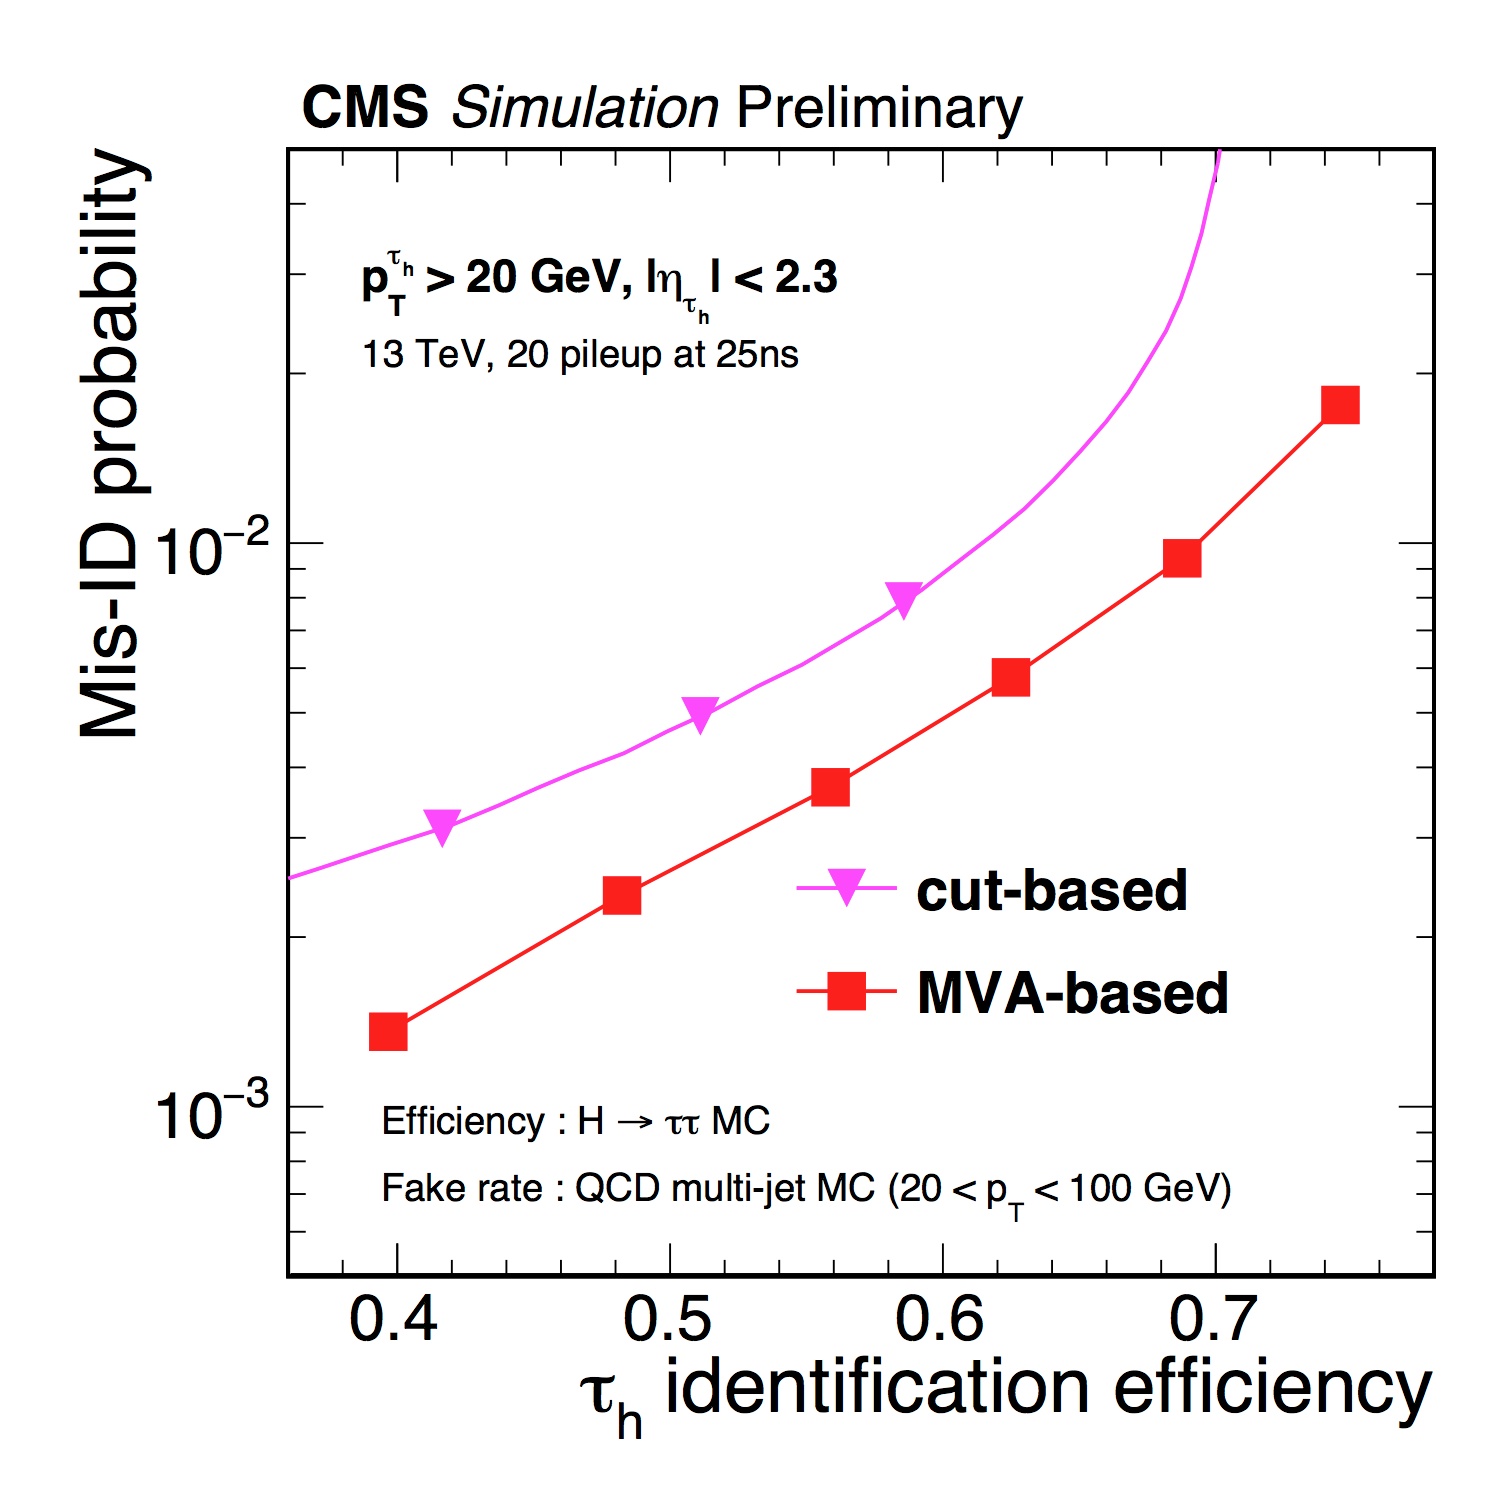
\includegraphics[width=0.7\textwidth]{./Objects/Plots/TauIsolationPlot.png}
\caption{Something about tau isolation}
\label{fig:tau_iso_efficiency}
\end{figure}

\subsection{Differences between Run 1 and Run 2}
\label{sec:objects_taus_diff}
Broadly speaking the algorithm used for hadronic tau reconstruction during Run 1
was similar to the Run 2 algorithm described earlier in this section. However, during
Run 1 strips were reconstructed using a fixed size of $0.05 \times 0.20$ in $\eta \times \phi$.
The dynamic size used in Run 2 was introduced to mitigate the effects of secondary particles
with low \pT and multiple \APelectron\Pelectron conversions, resulting in particles ending up outside of 
the strip window and making the hadronic tau seem less isolated than it actually is.
SOMETHING ABOUT Jet->Tau FAKE RATES AND e->TAU Misidentification



